\documentclass[a4paper,11pt]{article}
\usepackage{exptech}
\usepackage{textcomp}
\usepackage{graphicx}
\usepackage{array}
\usepackage[babel=true]{csquotes}
\usepackage{url}
\usepackage{hyperref}
\usepackage{wrapfig}
\usepackage[export]{adjustbox}
\usepackage{titletoc}

%\titlecontents{subsection}[3.8em]{}{}{}{}[\addvspace{-0.5pt}]
\hypersetup{
  pdftitle={Avalon - Rapport de planification}, % title
  pdfnewwindow=true, % links in new window
  colorlinks=true, % false: boxed links; true: colored links
  linkcolor=black, % color of internal links (change box color with linkbordercolor)
  citecolor=cyan, % color of links to bibliography
  filecolor=cyan, % color of file links
  urlcolor=cyan % color of external links
}

\title{
  \textbf{Avalon}\\
  Rapport de planification
}
\markright{Avalon - Rapport de conception }
\author{
\begin{minipage}{0.4\textwidth}
	\begin{flushleft} \large
		\emph{Auteurs :}\\
		Alexandre \textsc{Audinot}\\
		Julien \textsc{Bouvet}\\
		Thierry \textsc{Gaugry}\\
		Nicolas \textsc{Hurman}\\
		Alexandre \textsc{Leonardi}\\
	\end{flushleft}
\end{minipage}
\begin{minipage}{0.4\textwidth}
	\begin{flushright} \large
		\emph{Encadrants :} \\
		Valérie \textsc{Gouranton}\\
		Ronan \textsc{Gaugne}\\
		Bruno \textsc{Arnaldi}\\
		Willy \textsc{Allègre}\\
		Jean-Paul  \textsc{Departe}\\
	\end{flushright}
\end{minipage}
}

\date{06 Février 2015}

\begin{document}
\maketitle
\thispagestyle{empty}

\begin{figure}[h!]
   \begin{minipage}{0.3\linewidth}
      
\includegraphics[scale=0.9]{3-Planification/img/logo_insa.jpeg}
   \end{minipage} 
   \begin{minipage}{0.2\linewidth}
      \centering
      
\includegraphics[scale=0.5,left]{3-Planification/img/logo_irisa.jpg}
   \end{minipage}\hfill
   \begin{minipage}{0.2\linewidth}
      
\includegraphics[scale=0.9]{3-Planification/img/logo_kerpape.png}
   \end{minipage}
\end{figure}

\newpage
\tableofcontents
\pagebreak

\section{Introduction}

% Annonce plan
% Visite kerpape
% Rencontre clients
\begin{wrapfigure}{r}{0mm}
	\centering
	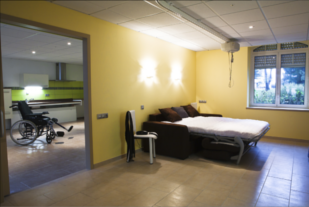
\includegraphics[scale=1]{1-PreEtude/img/appt_tremplin_intro.png}
\end{wrapfigure}
Notre projet consiste en la modélisation d'appartements tremplins en 3D pleinement interactifs, dans lesquels des personnes handicapées pourront évoluer et apprendre à se servir des différents équipements de domotique présents. 
Le projet est proposé par le centre de rééducation de Kerpape et par l'IRISA, ce qui lui confère un intérêt particulier à nos yeux car le commanditaire est extérieur à l'école, et le projet répond donc au besoin d'un véritable client de la même manière que le ferait un projet rencontré dans notre vie professionnelle. 
Ainsi, nous avons eu l'occasion de nous entretenir avec Willy Allègre et Jean-Paul Departe, ingénieurs de Kerpape à l'origine du projet, tout d'abord lors d'une conférence téléphonique pendant laquelle ils nous ont décrit ce qu'ils attendaient de l'application. Par la suite, un déplacement au centre de Kerpape nous a permis de parfaire l'image que nous nous faisons du résultat attendu et de compléter le cahier des charges de la future application. \newline

\begin{wrapfigure}{l}{0mm}
	%\cite{archeologie}
	\centering
	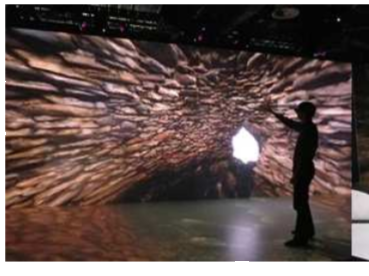
\includegraphics[scale=0.5]{1-PreEtude/img/rv_2.png}
\end{wrapfigure}
Au cours de cette étude de pré-spécifications, nous commencerons par définir plus précisément le contexte de notre projet, en tentant de cerner ce qu'est la réalité virtuelle et son importance dans le domaine de la santé. 
Nous présenterons ensuite le cahier des charges en deux parties, d'abord d'un point de vue fonctionnel, les différentes fonctions qui sont attendues de notre applications, et ensuite d'un point de vue technique, les différentes contraintes que nous aurons à respecter. 
Après cela nous décrirons, dans l'étude fonctionnelle, les différents scénarios types qui nous ont été proposés par Kerpape et auxquels les patients devront pouvoir être confrontés. 
Puis nous spécifierons les différents logiciels à notre disposition ainsi que les différents matériels, et les périphériques que nous prévoyons de rendre utilisables. 
Enfin, nous ébaucherons une planification prévisionnelle du travail à fournir tout au long de l'année. 
\pagebreak
Pour notre projet, nous n'allons pas utiliser une approche orientée objet classique, avec une modélisation UML totale des classes et de leurs interactions : travaillant avec Unity, nous devons adopter son paradigme de développement qui est basé sur de la programmation par composants.

Dans un modèle de programmation par composants, le but est de séparer au maximum chaque entité (composant) pour que son couplage avec les autres composants soit le plus faible possible. Les composants communiquent entre eux à l'aide d'interfaces simplifiées. Ils peuvent émettre et s'abonner à des évènements, tout comme les objets classiques, la différence étant que c'est leur principal mode d'interaction.

Un composant regroupe un ensemble de fonctionnalités proches, un peu comme un namespace pourrait le faire. Là où une approche simplement orientée objet se base sur des actions (équivalent de verbes en français), suivant le modèle \enquote{cible.action()}, la programmation orientée composants découpe le logiciel en une multitude de briques logicielles qui sont des boîtes noires pour le reste du projet. Il est tout à fait possible de développer des composants avec une méthode de programmation orientée objet, la contrainte étant que chaque composant soit totalement indépendant.

Dans le cas d'Unity qui est le nôtre, nous partons du graphe de scène qui contient un ensemble de \enquote{Game objects}. Ces game objects correspondent à des éléments de la vue 3D, comme une porte ou un interrupteur. C'est l'entité de base de Unity, il n'en existe pas de plus bas niveau. Chaque game object se voit associé une liste de composants, comme des matériaux, des lumières, des maillages, des animations... La famille de composants qui nous intéresse ici est celle \enquote{Script}.

Les composants \enquote{Script}, dans notre cas, sont des classes écrites en C\# qui étendent MonoBehaviour pour apporter une dimension dynamique supplémentaire aux objets ; un objet peut se voir associer plusieurs scripts. On pourrait par exemple imaginer un script qui permet de lever ou de baisser les volets, et un autre permettant de mettre en valeur l'objet activé en changeant la couleur de son matériau. Ces deux scripts peuvent être attachés à chaque volet de l'appartement, tandis que le second peut être réutilisé tel quel pour la télévision, une porte ou tout autre objet.

Chaque composant de type script peut redéfinir plusieurs méthodes pour effectuer ses actions. Il s'agit essentiellement de méthodes telles que \enquote{Update} qui sont appelées régulièrement, par exemple à chaque nouvelle image.

Les variables publiques des scripts apparaissent dans Unity comme des propriétés, modifiables directement dans l'inspecteur. On peut notamment avoir un champ \enquote{public xxxx Cible}, et depuis l'interface graphique, sélectionner un objet de type xxxx pour le faire glisser dans cette propriété.

Quand un script a besoin d'interagir avec d'autres objets que celui auquel il est attaché, il peut récupérer une référence vers un autre  object par la méthode précédente. Dans le cas où il ait besoin de le faire dynamiquement, il peut récupérer auprès du graphe de scène l'ensemble des objets auxquels sont attachés un script, ou bien un objet en particulier si celui-ci a été nommé ou taggé dans Unity.

Dans la suite de ce rapport, nous nous concentrerons donc sur les interfaces des divers composants ainsi que leurs interactions plus que sur leur fonctionnement interne (qui est trivial pour la plupart d'entre eux).

\pagebreak
\section{Architecture logicielle}
Pour ce projet, plusieurs logiciels nous ont été imposés. Cette partie détaille comment ces logiciels seront utilisés pour concevoir l'application.

\subsection{Unity}
\begin{figure}[h]
  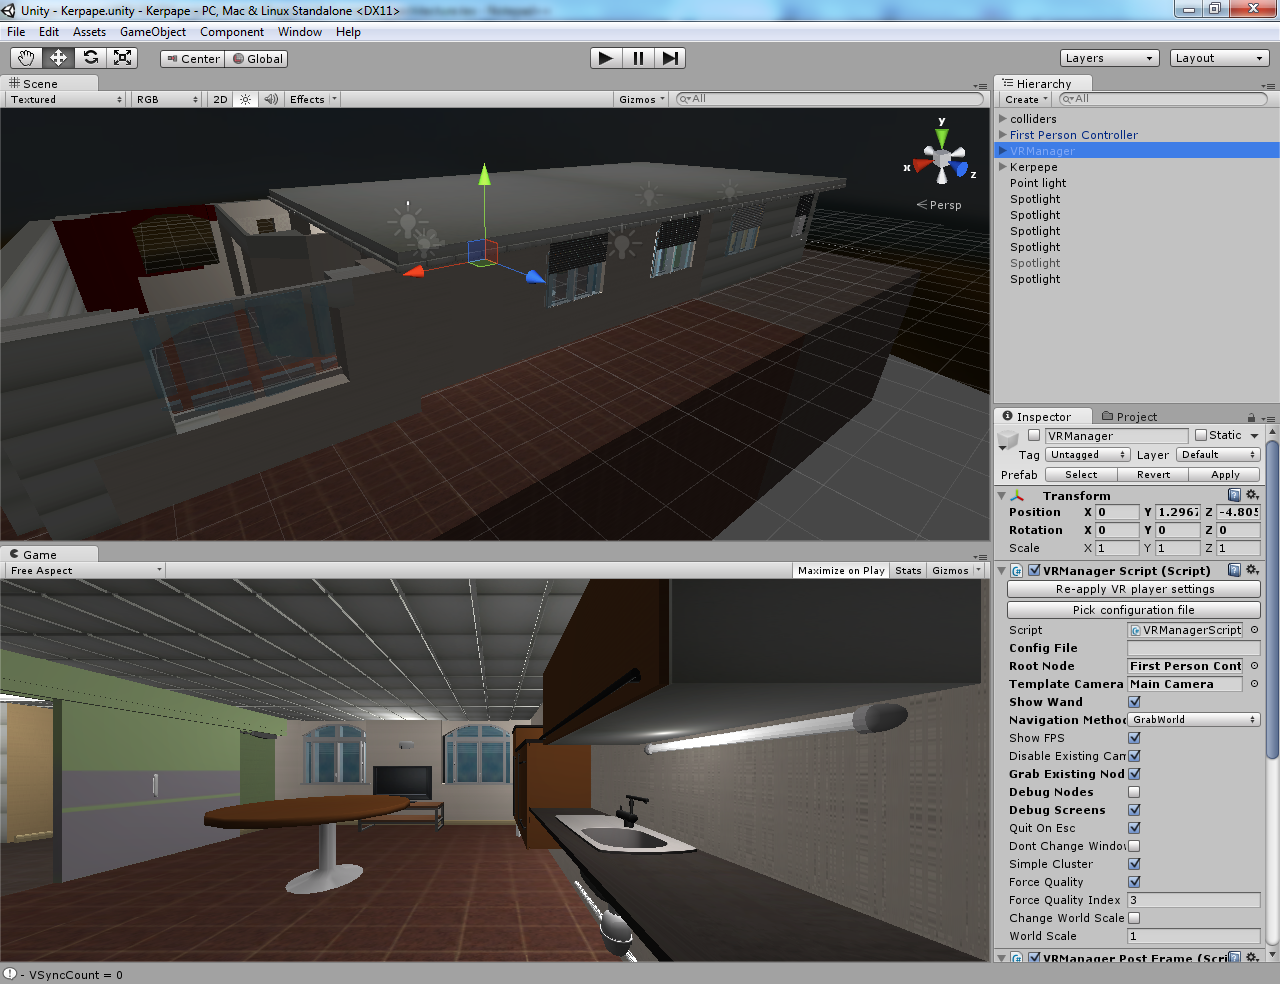
\includegraphics[width=1\textwidth]{4-conception/img/unity_screenshot.png}
  \caption{Capture d'écran : Unity}
  \label{unity}
\end{figure}

Unity est un moteur de jeu et environnement de développement. Bien que Unity donne la possibilité d'insérer des scripts pour gérer les objets plus en profondeur, il permet avant tout de créer une scène 3d. L'utilisateur peut se deplacer à l'interieur, en ayant des interactions avec l'environnement. Unity gère un certain nombre d'éléments, dont :
\begin{itemize}
        \item les colliders : représente les collisions engendrées par l'objet.
        \item les meshs : correspond à l'affichage des objets de la scène.
\end{itemize}


\subsection{MiddleVR}
\begin{figure}[h]
  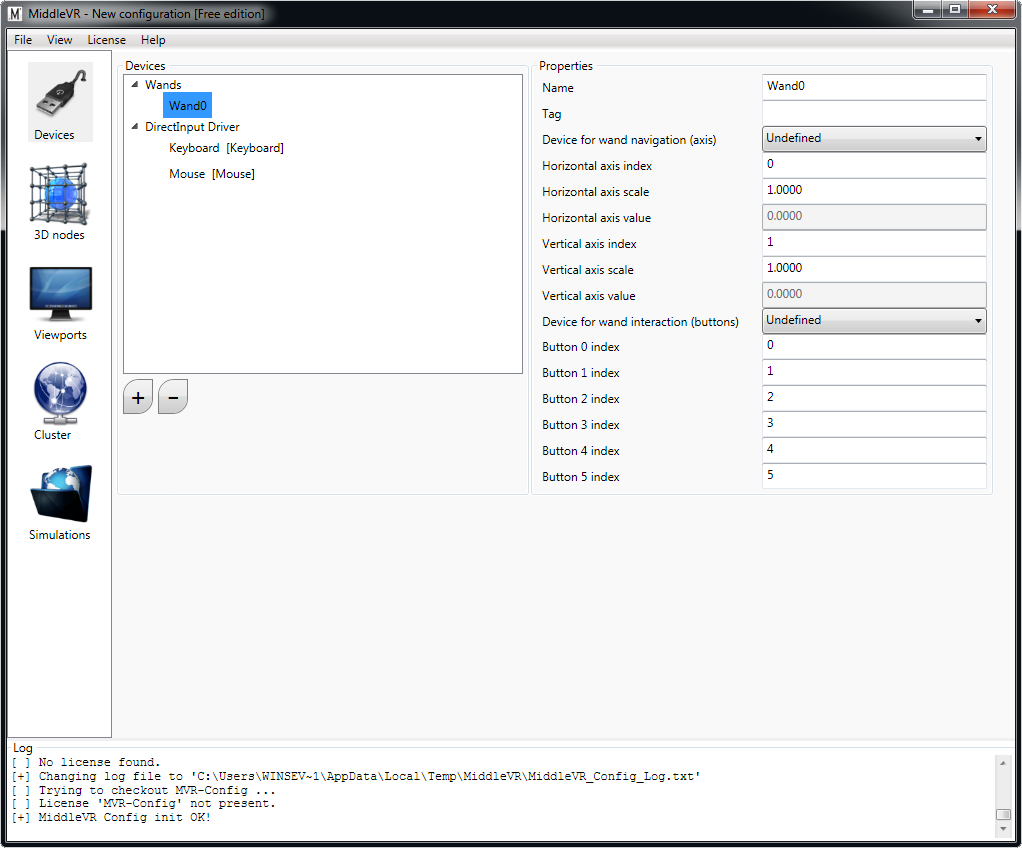
\includegraphics[width=1\textwidth]{4-conception/img/middlevr_screenshot.png}
  \caption{Capture d'écran : MiddleVR}
  \label{middlevr}
\end{figure}
MiddleVR est un plugin Unity utilisé pour s'abstraire des périphériques d'entrée/sortie. Il permet de créer un fichier de configuration contenant les informations sur les différents périphériques dont se servira l'application. Pour cela, MiddleVR possède sa propre interface et il n'est pas nécessaire d'écrire du code.
Pour récupérer les valeurs des périphériques dans Unity, on utilise le VRManager, qui sert d'interface entre Unity et MiddleVR.

\subsection{Script C\#}
Unity utilise des scripts en C\# pour réaliser des interactions plus poussées que de simples collisions. Ces scripts nous donnent la possibilité d'allumer ou éteindre une lumière, ou déplacer un objet par exemple. Ils sont l'unique type de code que nous allons produire dans ce projet, il devront donc gérer les différents modes d'apprentissage, ainsi que les scénarios d'utilisation.
Dans Unity, un script est attaché à un objet, il correspond à son comportement. Par exemple, un script attaché à un interrupteur va indiquer ce qu'il se passe lorsque le joueur appuie dessus. Il va commander le changement d'état de l'interrupteur, le changement de lumière (s'il commande la lumière d'une pièce) et éventuellement d'autres éléments selon le mode d'apprentissage.
\begin{figure}[h]
\centering
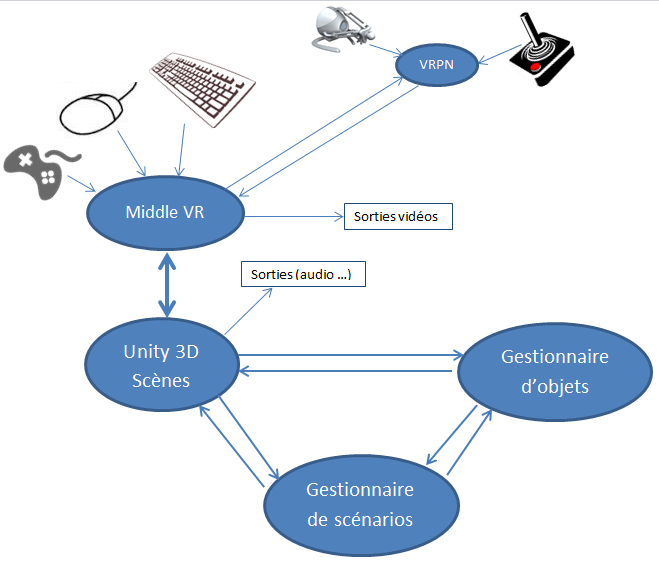
\includegraphics[width=1\textwidth]{4-conception/img/recap.png}
\caption{ Diagramme récapitulatif }
\label{recap}
\end{figure}

Dans la figure \ref{recap}, on peut noter que nous ne communiquons pas avec le VRPN nous-même, MiddleVR s'en charge à notre place. Pour plus d'informations sur le VRPN, voir http://www.middlevr.com/middlevr-for-unity/ ou notre rapport de pré-étude.

\pagebreak
\section{Lancement de l'application}

\begin{figure}[h]
\centering
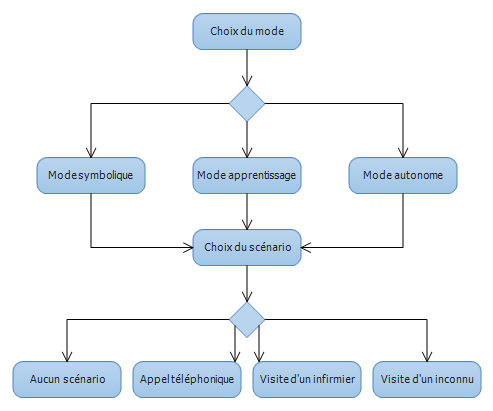
\includegraphics[width=1\textwidth]{4-conception/img/diagActivite.png}
\caption{ Diagramme récapitulatif }
\end{figure}

Au lancement du logiciel, l'utilisateur peut personnaliser la simulation par l'intermédiaire de plusieurs choix :

Tout d'abord, il peut choisir un mode d'apprentissage. Ces modes apportent de l'autonomie ou donnent des directions à l'utilisateur en lui donnant des indicateurs visuels sur ce qu'il peut faire. Voici les différents modes :
\begin{itemize}
\item Symbolique ;
\item Assisté ;
\item Autonome.
\end{itemize}


De plus, il est possible de jouer un scénario, pour forcer l'utilisateur à faire certains choix et interagir avec certains objets. Voici les différents scénarios :
\begin{itemize}
\item Appel téléphonique normal ;
\item Appel \textit{via} l'interphone d'une personne venant fréquemment (un infirmier par exemple) ;
\item Appel \textit{via} l'interphone concernant une visite inattendue.
\end{itemize}


Ces différents choix seront gérés par des scripts C\# de Unity, et plus précisement par le GameManager, décrit dans la partie "Modélisation" de ce rapport.


\pagebreak
\section{Modélisation}

\subsection{Diagramme des cas d’utilisations}


\subsection{Diagramme de classes C\#}

Sur le diagramme, une classe UI_Menu est présente. Elle représente les classes d'interface que nous utiliserons pour afficher des menus d'informations à l'utilisateur.
Nous utiliserons de préférence les classes rajoutées par la dernière version de MiddleVR (1.6.0), car ardaptées à la 3D et à la réalité virtuelle.
Cette version étant disponible seulement depuis la semaine précédente, nous n'avons pas eu l'occasion d'étudier l'architecture proposée pour cette partie.
Dans le cas où nous ne pourrions intégrer ces fonctionnalités, nous utiliserons une manière plus basique pour l'affichage, telle que des textures appliqués sur des plans.

\begin{figure}[p]
    \centering
    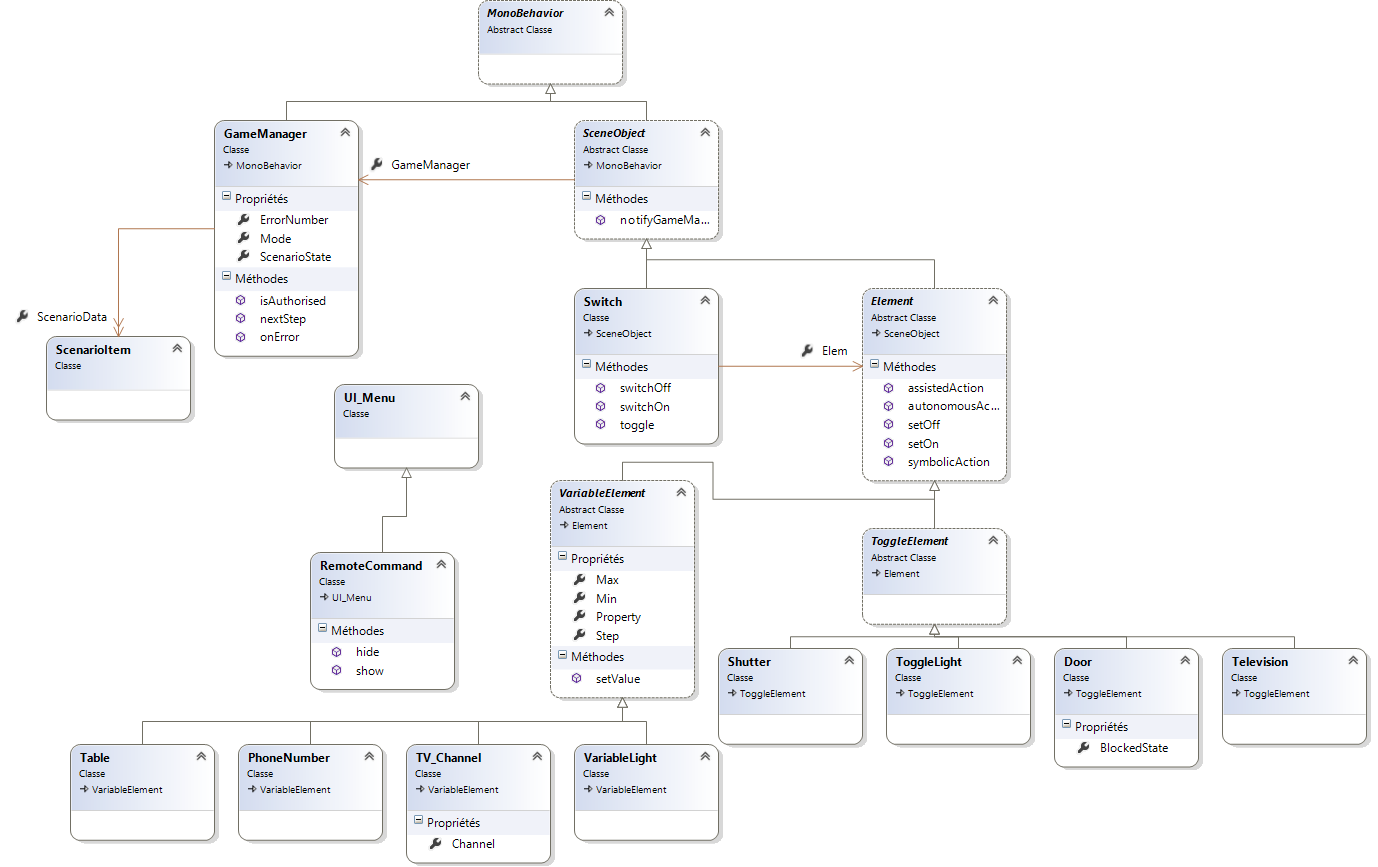
\includegraphics[width=0.8\textwidth]{img/diagClasses.png}
    \caption{Diagramme de classes}
    \label{fig:class_diagram}
\end{figure}
 
On distingue deux types d'éléments sur lesquels ont peut interragir : Ceux avec un état allumé/éteins, et ceux avec un état variable, comme la table et sa hauteur.
Tout les cas simples seront gérés par des ToggleElement. Les différences entre chaques sous classes se résument à des détails de l'objets.
Une lumière allumé ou éteinte n'est pas géré de la même manière que la hauteur d'un volet.
La classe VariableElement permet de gérer les GameObjects avec une valeur interne; il est possible de d'augmenter les variables de manière incrémentale ou de fixer une valeur directement.
Cette classe inclu une valeur minimale et maximale pour la valeur contrainte, ainsi qu'un pas de déplacement.
Ce pas permet de régler le changement de valeur à chaque clic; par exemple, on choisira 1cm dans le cas de la table, pour que le déplacement soit cohérent avec la réalité.

Ce modèle inclu aussi les spécificités relatives au différents éléments, comme la propriété BlockedState des portes qui permet de savoir où le mouvement de la porte à été stoppé la dernière fois, pour ralentir lors du prochain essai.

Toutes ces classes, comme \textit{VariableLight}, \textit{Shutter} ou \textit{Table},  ne disposent pas de variable modélisant leur état courant. 
Il faut prendre en compte que ce sont des scripts associé un objet 3D. 
La valeur actuelle (de hauteur dans le cas de la table par exemple) correspond à une ou plusieurs caractéristiques graphiques de l'objet.

La classe GameManager s'apparente dans l'utilisation à un singleton, bien que n'en étant pas un. 
Pour toutes les informations et les fonctionnalités non liées à un objet en particulier (souvent encapsulé dans un singleton dans un contexte objet), les developpeurs unity préconisent d'associer des scripts à un GameObject n'ayant pas d'éléments graphiques et ne contenant pas d'autres GameObject.
L'accès à ces éléments se fait via le nom du GameObject les contenant, ou via des tags référençant l'élément.

\pagebreak
\section{Conclusion}

Nous avons donc choisi une méthode fortement inspirée du cycle de production en V mais en la mêlant à des méthodes agiles pour pouvoir présenter le projet à nos clients régulièrement. Ainsi si chaque jalon du projet, représenté par un livrable à rendre, correspond à une étape de notre cycle en V, nous prévoyons en parallèle d'avancer le développement de l'application, en en présentant les itérations successives à Jean-Paul Departe et Willy Allègre. \newline

Ainsi, nos commanditaires peuvent valider notre avancée en quasi-temps réel. De plus, d'après l'audit réalisé sur Microsoft Project, nous disposons d'une planification correcte. Les différents livrables seront réalisés dans les temps et les estimations que nous avons faites tiennent compte des contre-temps que nous sommes susceptibles de rencontrer et devraient suffire à absorber les retards.

\end{document}
